\documentclass{article}

\usepackage[czech]{babel} 
\usepackage[utf8]{inputenc}
\usepackage[T1]{fontenc}
%\usepackage[IL2]{fontenc} % Different type of font for wierdos
\usepackage{graphicx} % Required for the inclusion of images
\usepackage{natbib} % Required to change bibliography style to APA
\usepackage{amsmath} % Required for some math elements 
\usepackage{amsfonts}
\usepackage{amssymb}
\usepackage{booktabs}
\usepackage{epstopdf}
\usepackage{multicol}
\usepackage{color}
\usepackage{float}
\usepackage[total={15.5cm,23.5cm}, top=2.5cm, left=3cm, includefoot]{geometry}
\usepackage[colorlinks=true,linkcolor = black, urlcolor = black, citecolor = black]{hyperref}
\usepackage{enumitem}
\usepackage{subfig}
\usepackage[toc,page]{appendix}
\usepackage{hyperref} 
\usepackage{minted}
\usemintedstyle{vs}

%For importing Matlab code
\usepackage{listings}
\usepackage{color} %red, green, blue, yellow, cyan, magenta, black, white
\definecolor{mygreen}{RGB}{28,172,0} % color values Red, Green, Blue
\definecolor{mylilas}{RGB}{170,55,241}

%\setlength\parindent{0pt} % Removes all indentation from paragraphs
\setlength{\parindent}{4em}
%----------------------------------------------------------------------------------------
%	DOCUMENT INFORMATION
%----------------------------------------------------------------------------------------

\author{Jindřich \textsc{Wolf}} % Author name

\date{\today} % Date for the report

%Definition of title page: 

\newcommand{\maketitlepage}{
	\begin{center}
	\thispagestyle{empty}
	
	{\LARGE{Západočeská univerzita v Plzni}}\\[.7em]
	{\LARGE{Fakulta aplikovaných věd}}\\[.7em]
	{\LARGE{Katedra kybernetiky}} \\[8cm]

	\begin{figure}[H]
		\centerline{
\includegraphics[scale=0.7,trim = 0cm 0cm 0cm 10cm]{./pdfs/FAV_logo.pdf}}
	\end{figure}
	{\Huge\textsc{Referát č.1 - Název semestrálky}}\\[.5em]
	{\Large\textsc{Plný název předmětu}}\\
	{\textsc{Zkratka katedry/zkratka předmětu (KKY/MATL)}}
	\end{center}	
	\vfill
	

	\begin{flushright}
		\Large{Jindřich Wolf}\\
		\Large{dd.mm.yyyy}
	\end{flushright}
}

%----------------------------------------------------------------------------------------



\renewcommand{\listingscaption}{Kód}
%\renewcommand{\thesubsubsection}{\thesubsection.\alph{subsubsection}}
%\addbibresource{sablona.bib}




%----------------------------------------------------------------------------------------  

\begin{document} 
\maketitlepage

\section{Zadání}
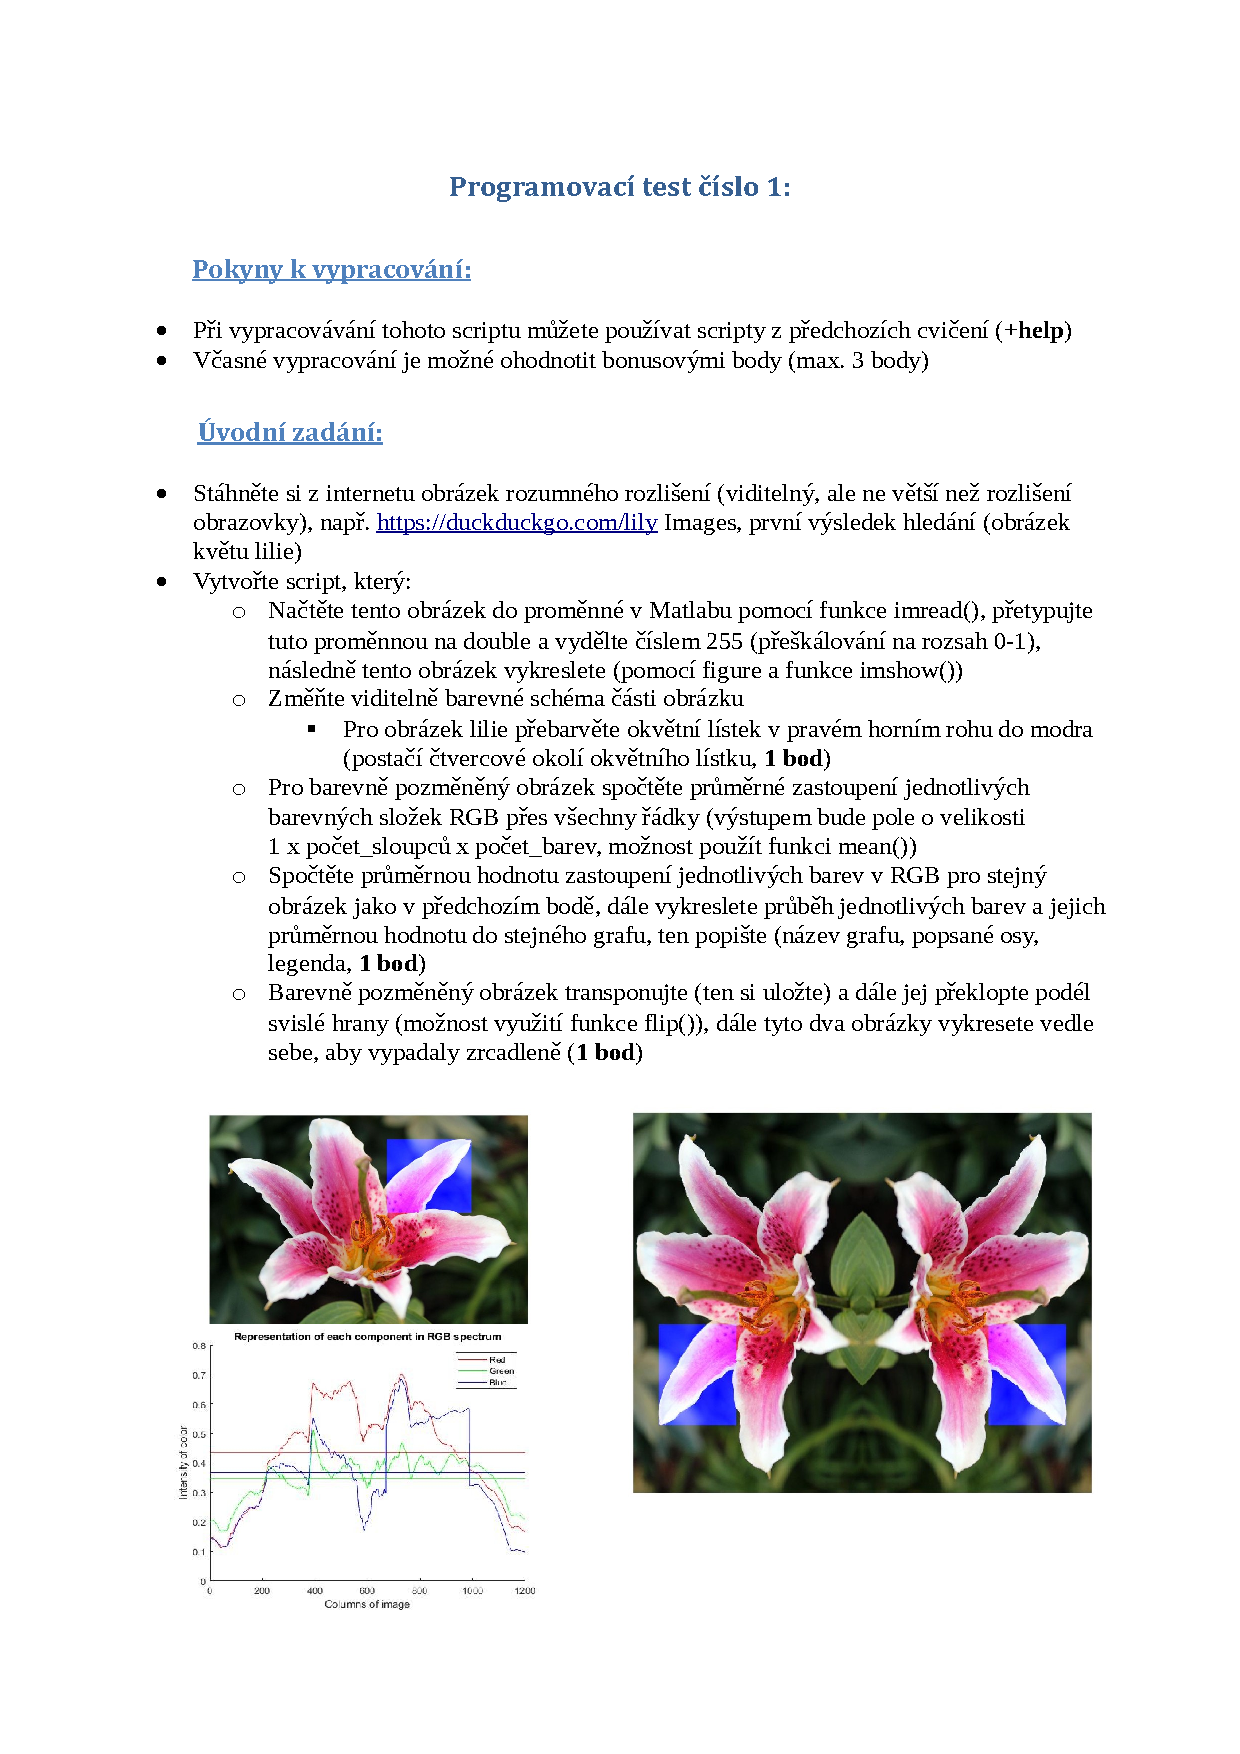
\includegraphics[scale=0.73]{./pdfs/Programovaci_test_1_pripravny.pdf} %scale- magic constant so your title and .pdf fits on same page
\newpage
\begin{center}
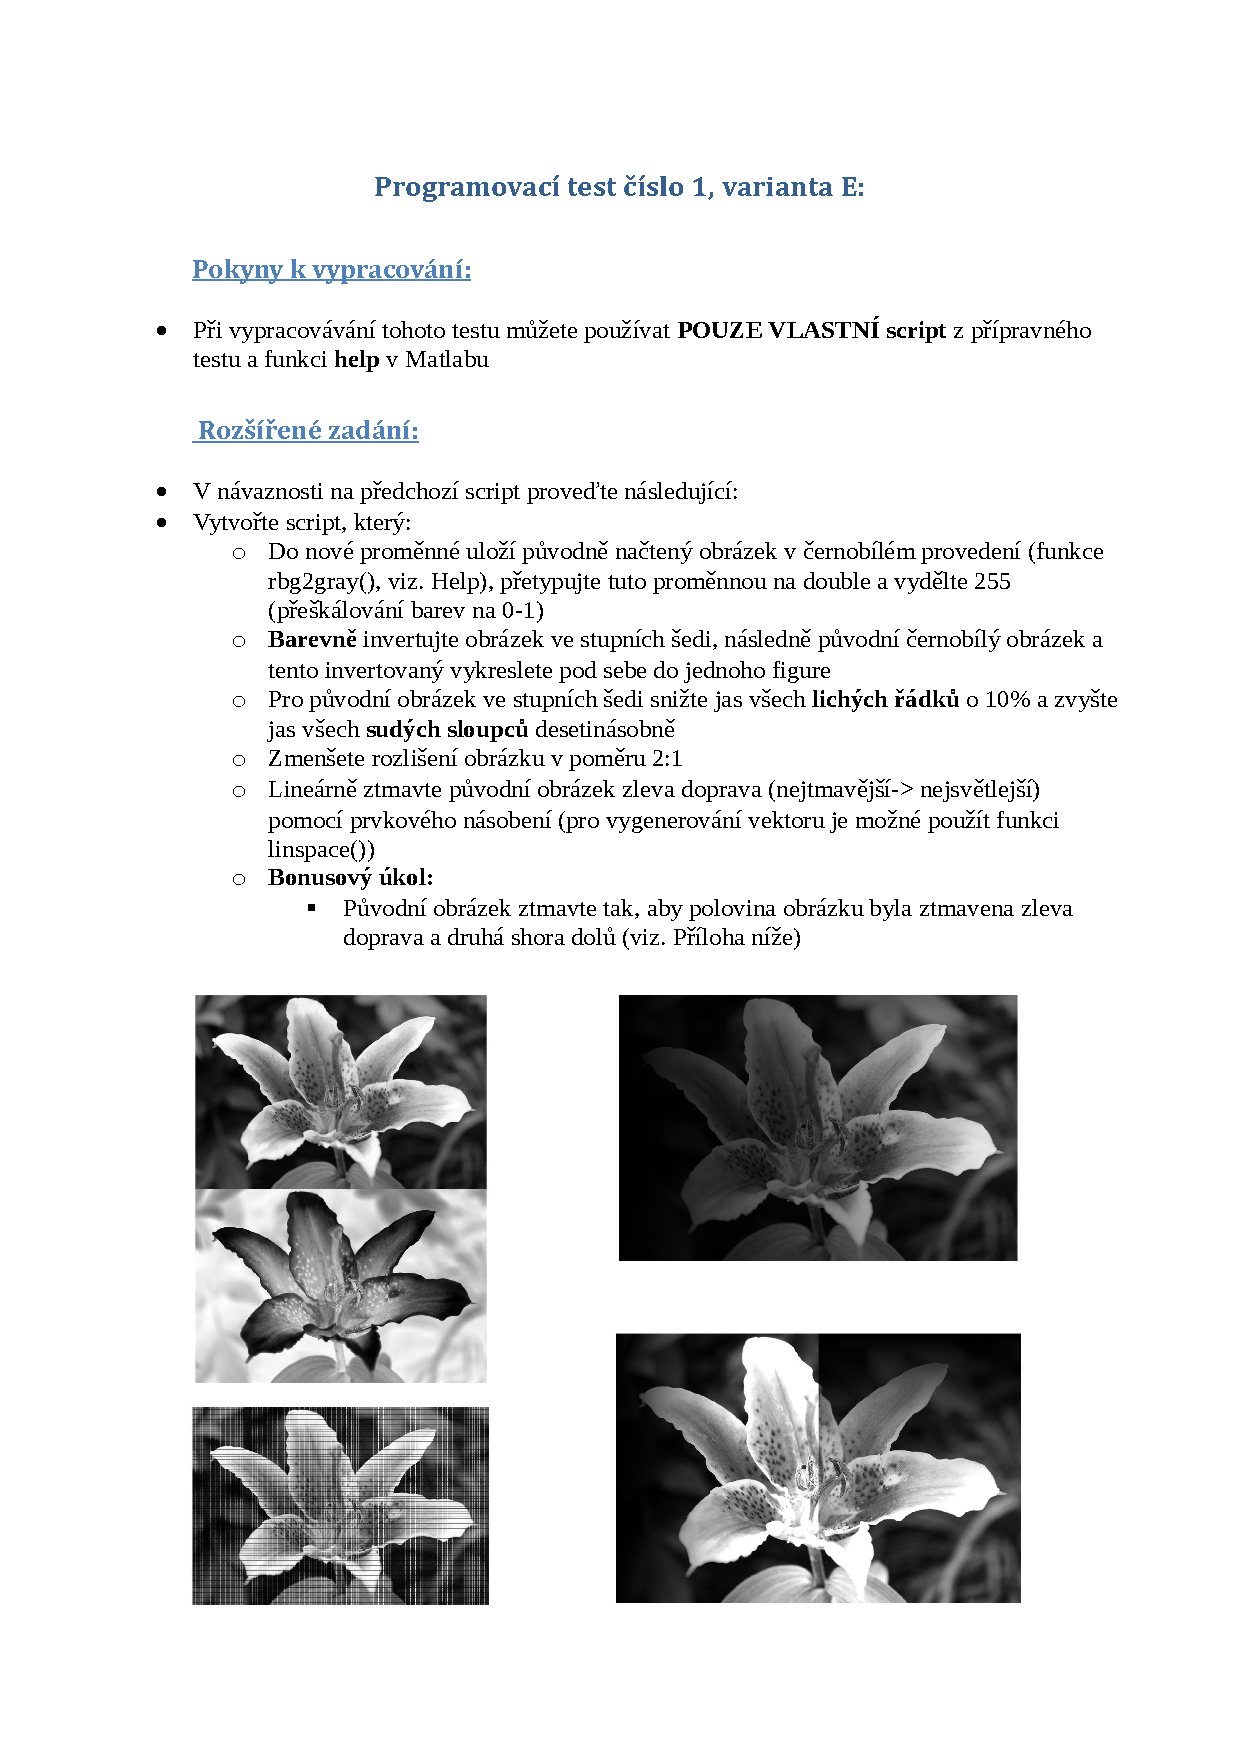
\includegraphics[scale=0.73]{./pdfs/Programovaci_test_1_rozsireny.pdf}
\end{center}

\newpage
\section{Postup řešení}
%First paragraph won't be indented because of czech language norms
\par Může být pár slov obecně o daném problému... pro nás kraťoučký text o tom, proč to píšeme přes script, proč třeba nepoužijeme pomocnou funkci, jaké nástroje kdyžtak používáme a v jakém programu. Je vhodné vkládat i \verb|ukázky kódu| \verb^tady vlastně může být jakýkoliv nepísmenný znak lol^ nebo i \mint{html}|<h2>Something <b>here</b></h2>| přes mint, ale ten už dělá odstavce :(
\par Lorem ipsum dolor sit amet, consectetuer adipiscing elit. Nulla est. Aliquam erat volutpat. Pellentesque pretium lectus id turpis. Nullam sit amet magna in magna gravida vehicula. Nunc dapibus tortor vel mi dapibus sollicitudin. Nunc auctor. Donec iaculis gravida nulla \eqref{stav}.
\subsection{Řešení první poloviny zadání}
\par Pellentesque habitant morbi tristique senectus et netus et malesuada fames ac turpis egestas. Sed elit dui, pellentesque a, faucibus vel, interdum nec, diam. Fusce nibh. Etiam egestas wisi a erat. In rutrum. In enim a arcu imperdiet malesuada.
\subsubsection{Import a úprava obrázku}
\par Nulla quis diam. Vestibulum fermentum tortor id mi. Integer in sapien. Proin in tellus sit amet nibh dignissim sagittis. Duis sapien nunc, commodo et, interdum suscipit, sollicitudin et, dolor. Praesent in mauris eu tortor porttitor accumsan. Quis autem vel eum iure reprehenderit qui in ea voluptate velit esse quam nihil molestiae consequatur, vel illum qui dolorem eum fugiat quo voluptas nulla pariatur? Sed elit dui, pellentesque a, faucibus vel, interdum nec, diam. Etiam dui sem, fermentum vitae, sagittis id, malesuada in, quam. 
\par Class aptent taciti sociosqu ad litora torquent per conubia nostra, per inceptos hymenaeos. Sed elit dui, pellentesque a, faucibus vel, interdum nec, diam. Donec ipsum massa, ullamcorper in, auctor et, scelerisque sed, est. Excepteur sint occaecat cupidatat non proident, sunt in culpa qui officia deserunt mollit anim id est laborum. Etiam sapien elit, consequat eget, tristique non, venenatis quis, ante. Fusce suscipit libero eget elit.
\begin{figure}[H]
	\centerline{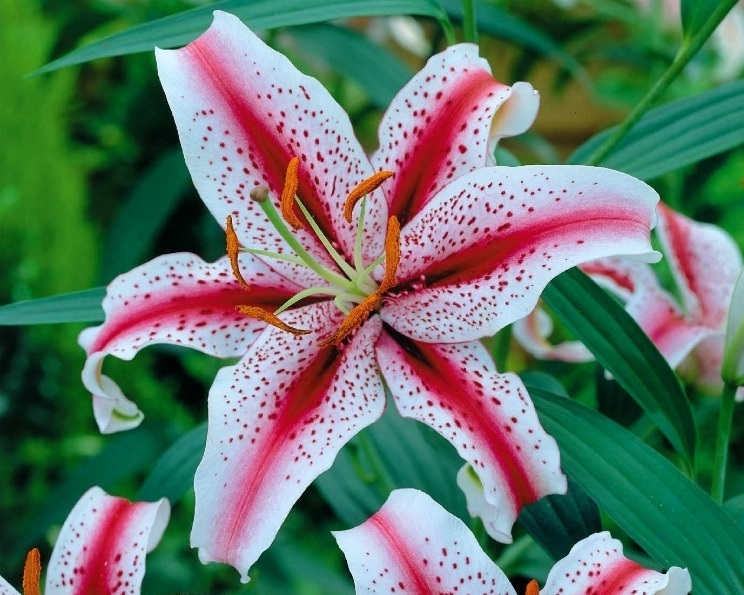
\includegraphics[scale=0.3]{./pics/lilie.jpg}}
	\caption{Užitečný popis obrázku říkající, co na něm mám vidět a čeho je to třeba výsledek.}
\end{figure}

\section{Matlab kód}

%barevný vkládání kódu
\begin{listing}[H]
    \inputminted[firstline=1, lastline=10]{matlab}{appendices/week7.m}
    \caption{Část kódu}
\end{listing}

%nebarevný
\begin{listing}[H]
    \lstinputlisting[language=matlab, firstline=1, lastline=10]{appendices/week7.m}
    \caption{Jinak vložená část kódu}
\end{listing}


\subsubsection{Změna barevného schéma}
\par Aliquam erat volutpat. Proin mattis lacinia justo. Etiam posuere lacus quis dolor. Integer malesuada. Praesent vitae arcu tempor neque lacinia pretium. Mauris dolor felis, sagittis at, luctus sed, aliquam non, tellus. Curabitur sagittis hendrerit ante. In dapibus augue non sapien.

\par Usefull commands for future usage:
\begin{enumerate}
	\item One
    \begin{enumerate}
    	\item Two
        \item Three
        \item Four
    \end{enumerate}
	\item Five
    \item Six
\end{enumerate}
\par Without names of items:
\begin{itemize}
  \item One entry in the list
  \item Another entry in the list
\end{itemize}
\par Numbered equation
 \begin{equation} 
  	S= \frac{1}{1+CP}
  \end{equation}
\par Unnumbered equation %Same you can unnumber many other things in LateX, check it as first option
\begin{equation*}
  	T= \frac{CP}{1+CP}
  \end{equation*}
\par Matrix equations:
\begin{gather*} %Auotamtically align things to center, you can't redesign that
    \textbf{A} \otimes \textbf{B}= \left[\begin{array}{ccc} a_{11}\textbf{B} & \cdots & a_{1n}\textbf{B}\\ \vdots & \ddots & \vdots \\ a_{m1}\textbf{B} & \cdots & a_{mn}\textbf{B} \end{array}\right].
\end{gather*}
\par Et harum quidem rerum facilis est et expedita distinctio. Praesent in mauris eu tortor porttitor accumsan. Aliquam erat volutpat. Aliquam erat volutpat. Pellentesque habitant morbi tristique senectus et netus et malesuada fames ac turpis egestas. Phasellus rhoncus.

\begin{align*} %Align let's you choose how to align things with char &, so here I'm aligning by=
\left[\begin{array}{c} \dot{x}\\ \dot{y}\\ \ddot{x}\\ \ddot{y} \end{array}\right]=
\left[\begin{array}{cccc} 0 & 0 & 1 & 0\\ 0 & 0 & 0 & 1\\ 0 & 0 & 0 & 0\\ 0 & 0 & 0 & 0 \end{array}\right]
\left[\begin{array}{c} x\\ y\\ \dot{x}\\ \dot{y} \end{array}\right] + 
\left[\begin{array}{cc} 0 & 0\\ 0 & 0\\ 1 & 0\\ 0 & 1 \end{array}\right]
\left[\begin{array}{c} u_x \\ u_y \end{array}\right]
\end{align*}


\par How to write some special symbols within sentence $ {Is}_{easy}^{pretty} \text{ You just have to } \mathbf{BELIEVE} \quad \lambda $ and it goes on its own...
\begin{align*}
\mathbf{S}^{-1}(\mathbf{L})\mathbf{S}=\mathbf{J}=
\left[ 
\begin{array}{cccc}
\mathbf{J}_{n_1}(\overline{\lambda}_1)& &&  \\
 & \mathbf{J}_{n_2}(\overline{\lambda}_2) & & \\
& & \ddots & \\ 
&&&\mathbf{J}_{n_k}(\overline{\lambda}_k) \\
\end{array}\right],
\end{align*}
\begin{align}\label{stav} %\label makes you label that you can use within text that links you to this equation, check first paragraph at the end:
     \dot{x}(t)&= \textbf{A}x(t) + \textbf{B}u(t),\\
     y(t)&= \textbf{C}x(t) + \textbf{D}u(t), \nonumber
\end{align}

\par More examples:
\begin{align*}
\dot{\tilde{x}}_i&= \dot{x}_i = v_i =  \tilde{v}_i,\\
\dot{\tilde{v}}_i&= u_i = c\sum_{j=1}^{N}a_{ij}[(x_j- \Delta_j)- (x_i- \Delta_i)] +  c \gamma \sum_{j=1}^{N}a_{ij}(v_j- v_i),\\
\dot{\tilde{v}}_i&=  c\sum_{j=1}^{N}a_{ij}(\tilde{x}_j- \tilde{x}_i) +  c \gamma \sum_{j=1}^{N}a_{ij}(\tilde{v}_j- \tilde{v}_i).
\end{align*}

\begin{align*}
\left[\begin{array}{c} \dot{\tilde{z}}_1\\ \dot{\tilde{z}}_2\\ \vdots \\ \dot{\tilde{z}}_N \end{array}\right]&= 
\left[ 
\begin{array}{cccc}
 \tilde{\mathbf{A}}_1 & \mathbf{0}& \cdots  & \mathbf{0} \\
 \mathbf{0}  & \tilde{\mathbf{A}}_2 & & \vdots \\
  \vdots & & \ddots & \mathbf{0}\\
\mathbf{0} & \cdots & \mathbf{0} & \tilde{\mathbf{A}}_N
\end{array}\right]
\left[\begin{array}{c}{\tilde{z}}_1\\ {\tilde{z}}_2\\ \vdots \\ {\tilde{z}}_N \end{array}\right]
 - \mathbf{L} \otimes
\left[
\begin{array}{cccc}
 \tilde{\mathbf{B}}_1 & \cdots  & \mathbf{0} \\
 \mathbf{0}  &\ddots  & \vdots \\
  \vdots &  & \mathbf{0}\\
\mathbf{0} & \cdots  & \tilde{\mathbf{B}}_N
\end{array}\right]
\left[
\begin{array}{cccc}
 c\mathbf{ K} & \mathbf{0}  \cdots&  & \mathbf{0} \\
  \vdots & \ddots & &\vdots \\
\mathbf{0} & \cdots &   \mathbf{0} & c \mathbf{K}
\end{array}\right]
\left[\begin{array}{c}{\tilde{z}}_1\\ {\tilde{z}}_2\\ \vdots \\ {\tilde{z}}_N \end{array}\right], \\[15pt]
\dot{\tilde{z}}&= (\mathbf{I}_n \otimes \tilde{\mathbf{A}} - c \mathbf{L} \otimes \tilde{\mathbf{B}} \mathbf{K})\tilde{z}= \tilde{\mathbf{A}}_c \tilde{z}.
\end{align*}

\par Multiple figures: \\
\begin{figure}[H]%
    \centering
    \subfloat[ $c=1$]{{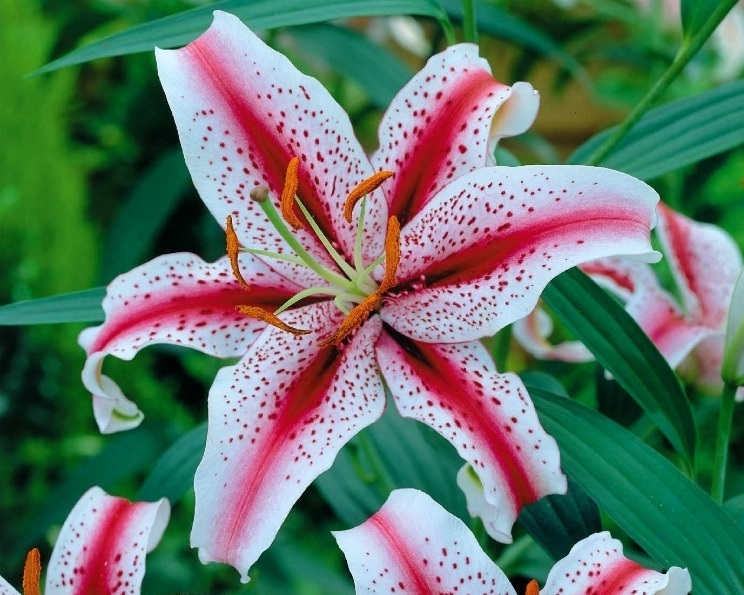
\includegraphics[height=3cm]{./pics/lilie.jpg} }}%
    \\
    \subfloat[$c=2$]{{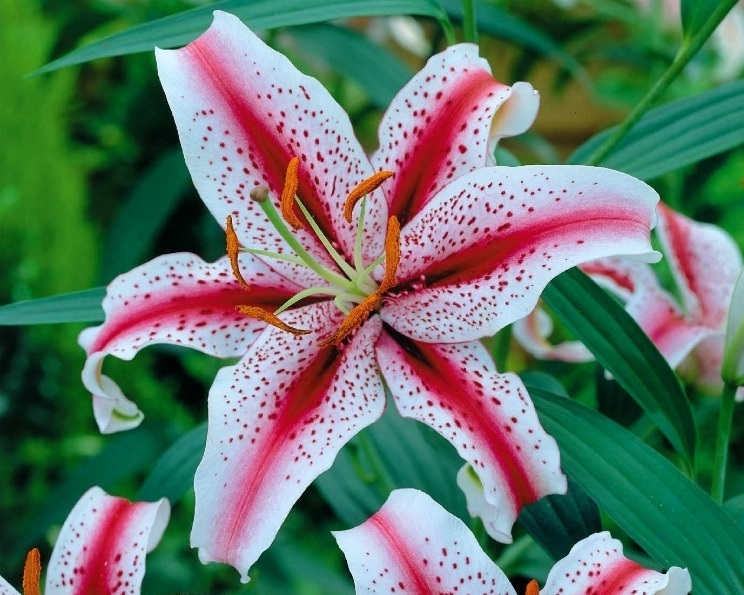
\includegraphics[height=3cm]{./pics/lilie.jpg} }}%
\\
\subfloat[$c=5$]{{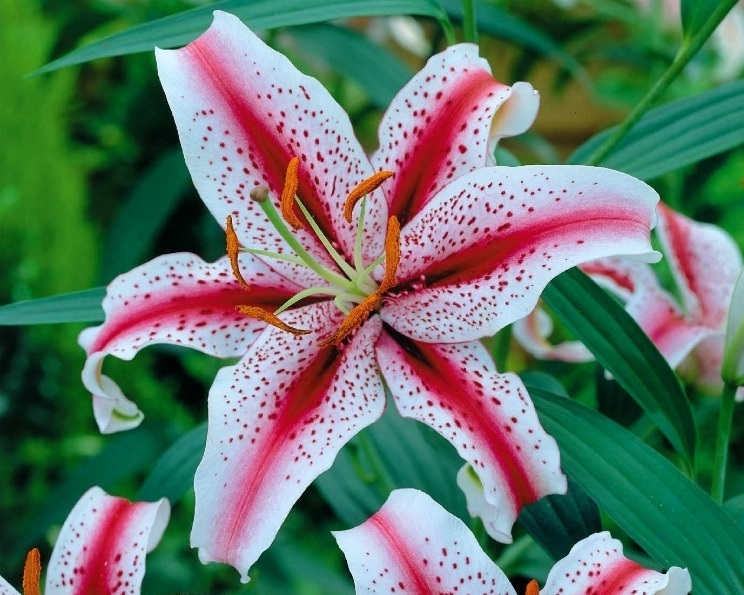
\includegraphics[height=3cm]{./pics/lilie.jpg} }}%
    \caption{Průběh stavů systému popsaného vztahem \eqref{stav} s náhodnými počátečními hodnotami, kde byly voleny různé hodnoty parametru $c$. Světle modrá čára představuje časový průběh polohy leadra (referenční trajektorie). }%
\end{figure}

\par Pokud budeme uvažovat harmonický referenční signál $u_{ref.}=sin(t)$, volba návrhového parametru $c$ nabyde více na důležitosti.
\begin{figure}[H]%
    \centering
    \subfloat[ $c=1$]{{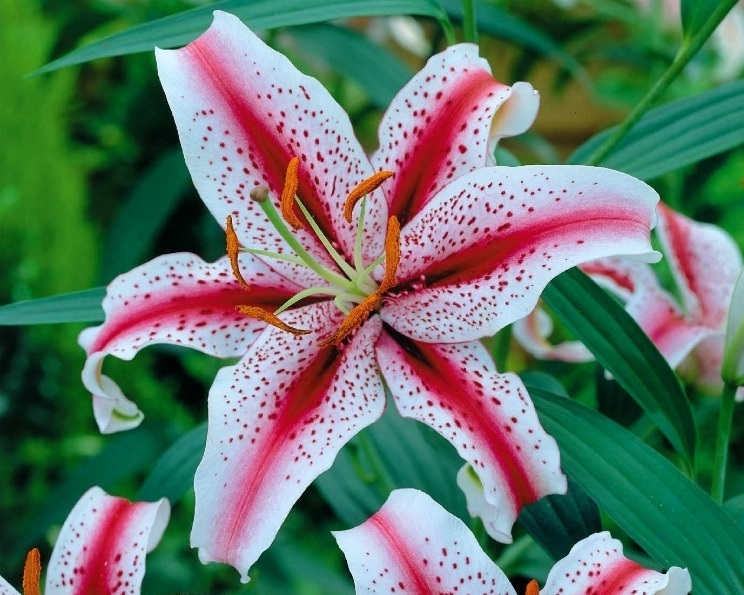
\includegraphics[width=6cm]{./pics/lilie.jpg} }}%
    \quad
    \subfloat[$c=2$]{{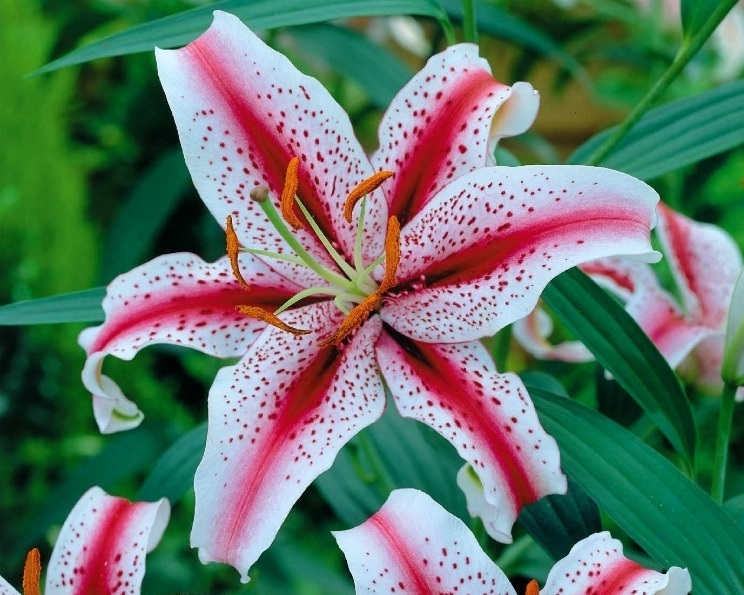
\includegraphics[width=6cm]{./pics/lilie.jpg} }}%
\\
\subfloat[$c=5$]{{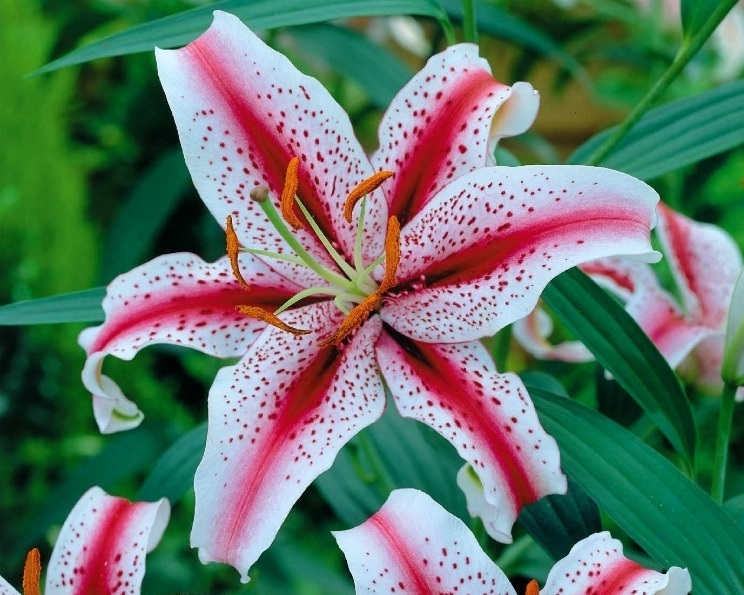
\includegraphics[width=6cm]{./pics/lilie.jpg} }}%
 \quad
    \subfloat[$c=15$]{{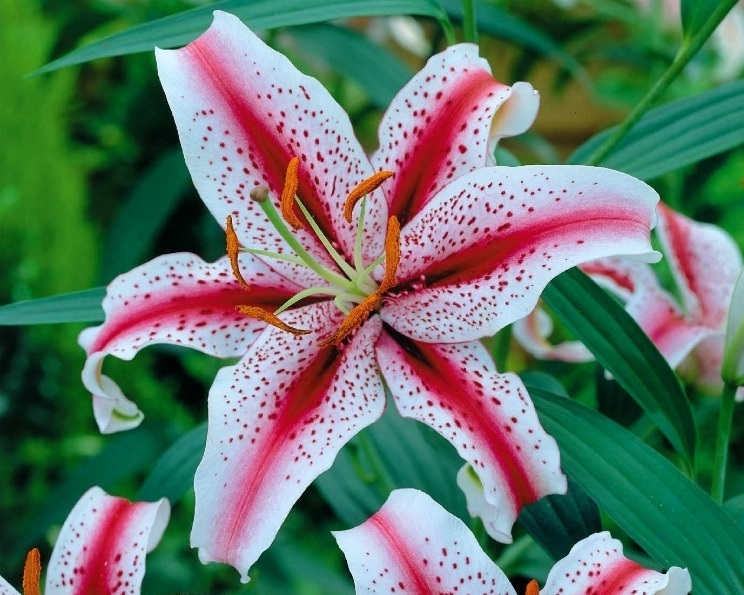
\includegraphics[width=6cm]{./pics/lilie.jpg} }}%
    \caption{Průběh stavů systému popsaného vztahem \eqref{stav} s náhodnými počátečními hodnotami, kde byly voleny různé hodnoty parametru $c$. Pro sledování nenulového referenčního signálu, který je v grafech reprezentován světle modrou čárou, je patrná důležitost správné volby parametru $c$.}
\label{ex1u}
\end{figure}

\newpage
\section{Závěr}
\par Aliquam ante. Phasellus enim erat, vestibulum vel, aliquam a, posuere eu, velit. Nam quis nulla. Class aptent taciti sociosqu ad litora torquent per conubia nostra, per inceptos hymenaeos. Integer tempor. Etiam quis quam. Integer vulputate sem a nibh rutrum consequat. Etiam dictum tincidunt diam. Etiam posuere lacus quis dolor. 
\par Nulla quis diam. Vestibulum erat nulla, ullamcorper nec, rutrum non, nonummy ac, erat. Praesent in mauris eu tortor porttitor accumsan. Pellentesque sapien.

\newpage
\appendix


\section{Never gonna give you up}
\begin{figure}[H]
	\centerline{
\includegraphics[scale=0.5]{./appendices/astley.jpg}}
	\caption{Never gonna let you down: \url{https://youtu.be/dQw4w9WgXcQ}.}
\end{figure}
\section{Užitečný odkazy}
\par Seznam důležitých odkazů k prostudování:\\
\begin{enumerate}
	\item \url{https://youtu.be/NN75im_us4k}
	\item \url{https://youtu.be/NPtJt4A7iOA}
	\item \url{https://youtu.be/dh-RUBbGZZA}
	\item \url{https://youtu.be/DouZ5VZQVuw}
	\item \url{https://youtu.be/jzG5Pkj08QU}
	\item \url{https://youtu.be/H_DWoIHD_7k}
	\item A zakončíme to zase Rickem a super videem :) \url{https://youtu.be/oT3mCybbhf0}
\end{enumerate}


\end{document}
